\section{Воздействие выхлопных газов автомобилей}
\begin{frame}{\insertsectionhead}
    \begin{columns}[onlytextwidth,c]
        \begin{column}{.50\linewidth}
          \footnotesize
          Выхлопные газы (или отработавшие газы) являются неоднородной смесью продуктов полного и неполного сгорания топлива. 
          Они состоят из различных газообразных веществ, большинство из которых токсичны.
        
          \smallskip

          Состав выхлопных газов включает огромное количество тяжелых металлов, которые зашлаковывают и 
          загрязняют организм. Так, например, свинец не удаляется из организма, а накапливается в 
          нем, поражая органы и ткани организма, нервную систему, желудочно-кишечный тракт.\cite{exhausts}            
        \end{column}
      
        \begin{column}{.45\linewidth}
          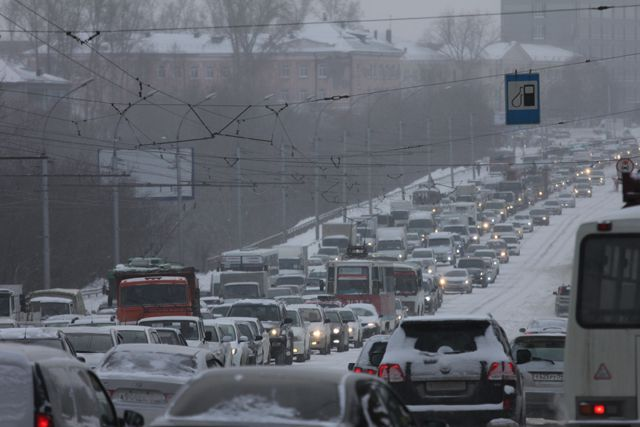
\includegraphics[width=\textwidth]{assets/probki.jpg}
        \end{column}
      
      \end{columns}
\end{frame}

\begin{frame}{\insertsectionhead}
    \begin{columns}[onlytextwidth]
        \begin{column}{.50\linewidth}
          \footnotesize
          Длительное воздействие выхлопных газов на человека:
          \begin{itemize}
              \item вызывает раздражение слизистых оболочек глаз и дыхательных путей;
              \item приводит к развитию заболеваний дыхательной системы(хронические бронхиты, рак);
              \item наносит вред головному мозгу, что может привести к развитию болезни Альцгеймера;
              \item отрицательно сказывается на нервной и сердечно-сосудистой системах.
          \end{itemize}            
        \end{column}
      
        \begin{column}{.47\linewidth}
          
\includegraphics[width=1.1\textwidth]{assets/chelovek-umeraet-ot-vihlopa.jpg}
        \end{column}
      
      \end{columns}
\end{frame}